\section{LLVM Structure} % Sections are added in order to organize your presentation into discrete blocks, all sections and subsections are automatically output to the table of contents as an overview of the talk but NOT output in the presentation as separate slides

%------------------------------------------------
\subsection{LLVM Compiler}
\begin{frame}{General Structure}
    \begin{figure}
	   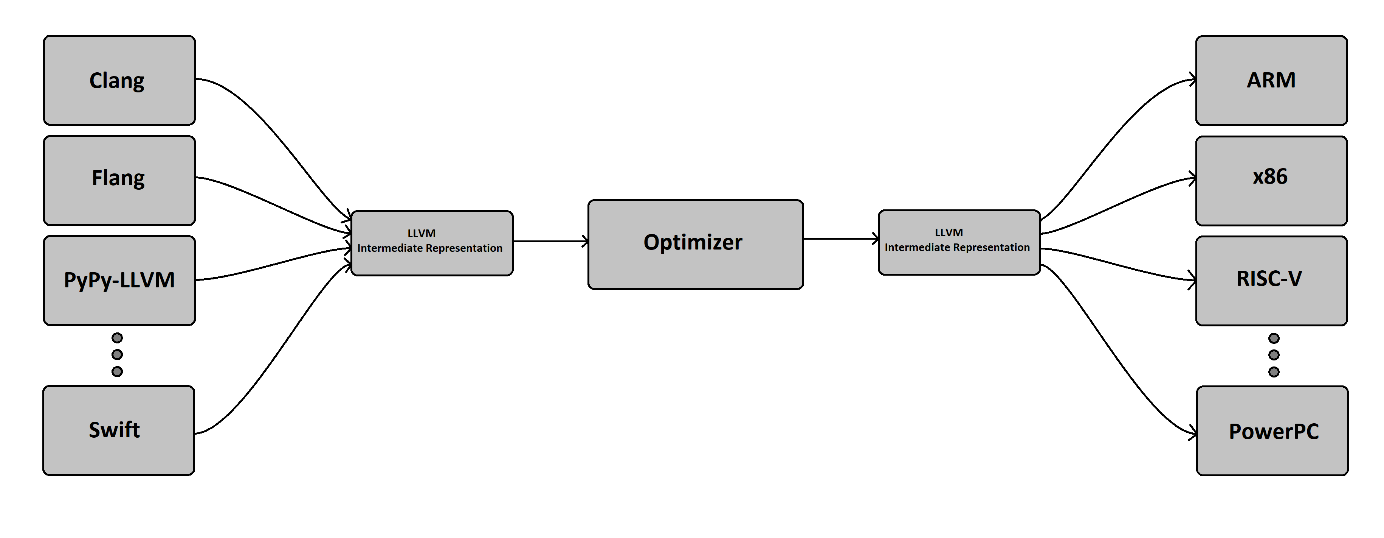
\includegraphics[width=0.8\linewidth]{llvm_diagram.png}
	   \caption{LLVM Frontend ve Backend}
	\end{figure}
\end{frame}

\subsection{LLVM Compiler Backend}
\begin{frame}{Backend}
    \begin{itemize}
        \item Instruction Selection
        \item Scheduling and Formation
        \item SSA based Machine Code Optimizations
        \item Register Allocation
        \item Prolog/Epilog Code Insertion
        \item Code Emission
        \item Linking
        
    \end{itemize}
\end{frame}

\begin{frame}{Instruction Selection Frameworks}
    \begin{itemize}
        \item FastISel
        \item SelectionDAG
        \item GlobalISel
    \end{itemize}
\end{frame}

\begin{frame}{SelectionDAG}
    \begin{enumerate}
    \item 
    Build initial DAG
    \item
    Optimize SelectionDAG
    \item
    Legalize SelectionDAG Types 
    \item
    Optimize SelectionDAG 
    \item
    Legalize SelectionDAG Ops 
    \item
    Optimize SelectionDAG
    \item
    Select instructions from DAG
    \item
    SelectionDAG Scheduling and Formation
    \end{enumerate}

	\begin{definition}
		A \alert{Directed Acyclic Graph (DAG)} is a directed graph with no cycles.
	\end{definition}
\end{frame}
